\documentclass[12pt]{article}

\usepackage[utf8]{inputenc}

% graphics
\usepackage{graphicx}
\usepackage[pdf]{graphviz}
\usepackage{amsmath}
\usepackage{amsfonts}
\usepackage{amssymb}
\usepackage{amsthm}
\usepackage{algorithm}
\usepackage{algpseudocode}
\usepackage{titling}
\usepackage{listings}
\usepackage{tikz}
\usetikzlibrary{automata,arrows,positioning,calc}



% citation
\usepackage{biblatex}
\addbibresource{report.bib}

% MACROS
\newcommand*{\QED}{\hfill\ensuremath{\square}}
\newcommand{\stirlingii}{\genfrac{\{}{\}}{0pt}{}}

\theoremstyle{definition}
\newtheorem{definition}{Definition}[section]

\newtheorem{theorem}{Theorem}
\newtheorem{lemma}[theorem]{Lemma}

\newcommand{\subtitle}[1]{%
  \posttitle{%
    \par\end{center}
  \begin{center}\large#1\end{center}
  \vskip0.5em}%
}

\newcommand*{\oh}{\frac{1}{2}}
% title
\title{Bayesian parameter synthesis of Markov population models}
\subtitle{Master Project on Modeling of Complex, Self-organizing systems}
\author{Huy Phung\\University of Konstanz}
\date{\today}

\setlength{\headheight}{23pt}
\setlength{\parindent}{0.0in}
\setlength{\parskip}{0.0in}


\begin{document}
\maketitle
\pagebreak
\tableofcontents
\pagebreak

%%%%%%%%%%%%%%%%%%%%%%%%%%%%%%%%%%%%%%%%%%%%%%%%%%%%%%%%%%%%%%%%%%%%%%%%%%%%%%%%%%%%%%%%%%%%%%%%%%%% 
\begin{abstract}
  We study the collective behavior of a bee colony. Each bee in a colony
  possibly stings after observing a threat in the surrounding environment, and
  warn other bees by releasing a special substance, pheromone. By sensing the
  pheromone released in the environment, other bees in the colony may also
  sting. However, since stinging leads to the termination of an individual bee,
  it reduces the total defense capability as well. With parametric Discrete-time
  Markov chain as the model, we study how the actions of a single bee change
  with regarding to the colony size of and pheromone amount. This project
  propose and discuss Bayesian methods to estimate parameters of bees population
  models. It shows that the proposed methods is scalable and can deliver
  estimations of model parameters.
\end{abstract}


%%%%%%%%%%%%%%%%%%%%%%%%%%%%%%%%%%%%%%%%%%%%%%%%%%%%%%%%%%%%%%%%%%%%%%%%%%%%%%%%%%%%%%%%%%%%%%%%%%%%
\section{Preliminaries}
\subsection{Discrete time Markov Chain}
Assume that each bee in a colony decides its next action (to sting or not to
sting) based only on the current state of the environment, and the number of
bees who sting or not sting can be modeled as a Markov process. To reduce the
complexity of the model, we make another assumption that the states of the bees
colony are observed after uniform time duration, hence the model is of
discrete-time. 

\subsubsection{Definition}
\begin{definition}[Discrete Time Markov Chain]
  A Discrete Time Markov Chain (DTMC) is a tuple $(S,\mathbf{P}, S_{init}, AP,
  L)$ \cite{baier2008principles} 
  \begin{itemize}
  \item $S$ is a countable non-emty set of \textit{states}
  \item $\mathbf{P}:S\times S \rightarrow [0,1]$ is the \textit{transition probability}
    function, s.t $$\sum_{s'\in S}\mathbf{P}(s, s') = 1$$
  \item $S_{init}: S \rightarrow [0,1]$ is the \textit{initial distribution},
    s.t  $$\sum_{s'\in S}S_{init}(s') = 1$$
  \item $AP$ is a set of \textit{atomic propositions}
  \item $L: S \rightarrow 2^{AP}$ is the labelling function on states.
  \end{itemize}
\end{definition}

The transition probability function in DTMC is given as a stochastic matrix $\mathbf{P}$,
which satisfies the following properties
\begin{itemize}
\item $\mathbf{P}$ is a square matrix.
\item $\mathbf{P}_{i,j} \in [0,1]$.
\item $\sum_j\mathbf{P}_{i,j} = 1$
\end{itemize}

\begin{definition}[Strongly Connected Component]
  Let $\mathcal{M}=(S,\mathbf{P}, S_{init}, AP,L)$ a DTMC. A subset $S'\subset
  S$ is strongly connected if and only if for every pair $s_1,s_2\in S'$ there
  is a path between $s_1$ and $s_2$ which consists of only of state in $S'$. If
  there exist no $S''\subseteq S$, such that $S\subset S''$ and $S''$ is
  strongly connected, then $S'$ is a \textit{Strongly Connected Component}, or
  \textit{SCC} in short.
\end{definition}

\begin{definition}[Bottom Strongly Connected Component]
  Let $\mathcal{M}=(S,\mathbf{P}, S_{init}, AP,L)$ a DTMC and $S'\in S$ a
  Strongly Connected Component. $S'$ is also a \textit{Bottom Strongly Connected
    Component}, or \textit{BSCC} for short, if and only if there exist no state
  $s \in S\\S'$ that is reachable from any state in $S'$.
\end{definition}

\subsubsection{Parametric Discrete-time Markov Chain}
In order to generalize the stochastic matrix to encompass unknown information of
the system, we introduce \textit{parametric DTMC}. Let $\theta =
(\theta_1,\ldots,\theta_n) \in [0,1]^n$, we represent each element in matrix
$\mathbf{P}$ as a polynomial function of $\theta$. Let $\mathbf{Pol}_\theta$ be the
set of polynomials $P: [0,1]^n \rightarrow [0,1]$. We define
\textit{parametric Discrete-Time Markov Chain}, or \textit{pMC} for short, as
follow:

\begin{definition}[Parametric DTMC]
  A parametric Discrete Time Markov Chain (pMC for short) is a tuple $(S,\theta,
  \mathbf{P}_\theta, S_{init}, AP, L)$
  \begin{itemize}
  \item $S$ is a countable nonemty set of \textit{states}
  \item $\theta$ is the set of model parameters
  \item $\mathbf{P}:S \times S \rightarrow \mathbf{Pol}_\theta$ is the \textit{transition probability}
    function that map a transition relation between two states to a polynomial
    function of $\theta$
  \item $S_{init}: S \rightarrow [0,1]$ is the \textit{initial distribution},
    s.t  $$\sum_{s'\in S}S_{init}(s') = 1$$
  \item $AP$ is a set of \textit{atomic propositions}
  \item $L: S \rightarrow 2^{AP}$ is the labelling function on states.
  \end{itemize}
\end{definition}
A concrete assignment of $\theta$ on pMC induces a DTMC. In this project, we
concern about the problem of data-informed estimation of model parameter $\theta$.

\subsubsection{Markov population model}
In the scope of this project we concern \textit{population} of a bee colony with
$N$ individuals initially.
We model the population of a bee colony using a pMC $\mathcal{M}=(S,\theta,
\mathbf{P}_\theta, S_{init}, AP, L)$ with the following properties:
\begin{itemize}
\item Each state $s\in S$ represent number of individuals in the bee colony.
\item There exists a set of terminal states $T\subset S$, such that $t$  is
  a BSCC for all $t\in T$, and $|T|=N+1$.
\end{itemize}
Assume we conduct a real biological experiment on a colony of $N$ bees. At the
end of the observation, we observes $N'$ bees $(0\leq N' \leq N)$ bees. Let
$tSCC_i\in T$ denotes the terminal states with $i$ bees left. As we conduct the
experiment with the same colony size multiple times, we get a probability
distribution over final states $T$.\\


\subsection{Bayesian inference}
\subsubsection{Bayesian parameter estimation}
Let $D$ be observed data. In statistical inference, we assume that the observed
data has a probability distribution of unknown parameter $\theta$, i.e
$D \sim P(D|\theta)$. In frequentist approach, the estimation
of $\theta$ based on long-run property, that is, given a large enough sample
size, expected value of parameter estimation $\hat{\theta}$ is equal to
$\theta$. Therefore, frequentist approach requires to gather a large amount of
data to deliver a close estimation $\hat{\theta}$. In Bayesian approach, we
reuse the information \textit{beliefs} gained from observed data to enhance the
accuracy of the estimation of $\hat{\theta}$. The main advantage of Bayesian
approach over frequentist approach is that it require less data to obtain an
estimation $\hat{\theta}$.\\
The beliefs obtained from prior knowledge of model parameter $\theta$ is
represented by \textit{prior
  distribution} $\pi(\theta)$.\\
Also, we have probability distribution of observed data, given parameter
$\theta$, $P(D|\theta)$. This is also called \textit{likelihood function}.\\
With Bayesian formula, we have
\begin{align*}
  \pi(\theta | D) = \frac{P(D|\theta)\pi(\theta)}{\int_\theta P(D|\theta)\pi(\theta)d\theta}
\end{align*}
$\int_\theta P(D|\theta)\pi(\theta)d\theta$ is called \textit{marginal
  distribution}. $\pi(\theta | D)$ is called \textit{posterior distribution}.
Computing posterior distribution is the essential part of Bayesian inference,
since it gives us the estimation of parameter $\theta$.

\subsubsection{Posterior conjugation}
Conjugated posteriors are special cases of Bayesian inference, in which the
prior and posterior distribution belongs to the same family of distribution.
Conjugated posteriors give us significant benefits
\begin{enumerate}
\item Tractability: we have analytical form of posterior distribution.
\item Computationally effective: updating model parameter is of linear time to
  the dimension of parameter.
\end{enumerate}
We consider two conjugated posterior: Binomial-Beta and Dirichlet-Multinomial
\begin{lemma}[Binomial-Beta Conjugation]
  Binomial distribution is conjugated to beta distribution.
\end{lemma}
\begin{proof}
  The observed data $D=(x_1,\ldots,x_n)$ is sampled from $Binomial(k, \theta)$ function
  \begin{align*}
    P(D|\theta) = \prod_{i=1}^n{k\choose x_i}\theta^{x_i}(1-\theta)^{k-x_i}
  \end{align*}
  The parameter $\theta$ is of $Beta(\alpha, \beta)$ distribution
  \begin{align*}
    \pi(\theta) = \theta^{\alpha-1}(1-\theta)^{\beta -1}
  \end{align*}
  We obtained:
  \begin{align*}
    \pi(\theta|D) &\sim P(D|\theta)\pi(\theta) \\
                  &\sim \theta^{\sum_{i=1}^n x_i}(1-\theta)^{nk -\sum_{i=1}^n x_i} \theta^{\alpha -1} (1-\theta)^{\beta-1} \\
                  &= \theta^{\alpha - 1 + \sum_{i=1}^n x_i}(1-\theta)^{\beta - 1 + nk -\sum_{i=1}^n x_i}
  \end{align*}
  Thus, the posterior is $Beta(\alpha + \sum_{i=1}^n x_i, \beta + nk -\sum_{i=1}^n x_i)$
\end{proof}
Generalize this conjugation, we also have Multinomial-Dirichlet conjugation.
\begin{lemma}[Multinomial-Dirichlet Conjugation]
  Multinomial distribution is conjugated to Dirichlet distribution.
\end{lemma}
\begin{proof}
  The observed data $D=(x_1,\ldots,x_n)$ is sampled from $Multinomial(n; \theta_1,\ldots,\theta_n)$ function
  \begin{align*}
    P(x_1,\ldots,x_n | N, \theta_0,\ldots,\theta_n) &= \frac{n!}{x_1!\ldots x_n!} \prod_{i=1}^n\theta_i^{x_i}
  \end{align*}
  The parameter $(\theta_1,\ldots,\theta_n)$ is
  $Dirichlet(\alpha_1,\ldots,\alpha_n)$
  \begin{align*}
    \pi(\theta_1,\ldots,\theta_n) = \frac{1}{\mathbf{B}(\alpha_1,\ldots,\alpha_n)}\prod_{i=1}^n\theta_i^{\alpha_i - 1}
  \end{align*}
  We obtain
  \begin{align*}
    \pi(\theta_1,\ldots,\theta_n|D) &\sim P(D|\theta)\pi(\theta) \\
                                    &\sim \prod_{i=1}^n\theta_i^{x_i} \prod_{i=1}^n\theta_i^{\alpha_i - 1} \\
                                    &\sim \prod_{i=1}^n\theta_i^{\alpha_i - 1 + \sum_{i=1}^n x_i}
  \end{align*}
  Thus, the posterior is $Dirichlet(\alpha_1 +  x_1,\ldots,\alpha_n
  +  x_n)$
\end{proof}
More detailed description in these cases can be found in \cite{tu2014dirichlet}
and \cite{baron2019probability}. We summarize the necessary results in the following table:
\begin{table}[H]
\begin{tabular}{lllll}
\cline{1-3}
\multicolumn{1}{|l|}{Likelihood} & \multicolumn{1}{l|}{Prior} & \multicolumn{1}{l|}{Posterior parameters} &  &  \\ \cline{1-3}
  \multicolumn{1}{|l|}{$Binomial(n, k)$}  & \multicolumn{1}{l|}{$Beta(\alpha, \beta)$}  & \multicolumn{1}{l|}{\begin{tabular}[x]{@{}c@{}}$\alpha' = \alpha + \sum_{i=1}^n x_i$\\$\beta' = \beta + nk -\sum_{i=1}^n x_i$\end{tabular}}  &  &  \\ \cline{1-3}
  \multicolumn{1}{|l|}{$Multinomial(n; \theta_1,\ldots,\theta_n)$}  & \multicolumn{1}{l|}{$Dirichlet(\alpha_1,\ldots,\alpha_n)$}  & \multicolumn{1}{l|}{$\alpha_i' =\alpha_i + x_i, 1 \leq i \leq n$}  &  &  \\ \cline{1-3}
                        &                        &                        &  & 
\end{tabular}
\end{table}

\subsubsection{Metropolis-Hastings algorithm}
In case the posterior distribution has no analytical form or its analytical form
is difficult to sample from directly, we use \textit{Metropolis-Hastings}
algorithm (\textit{MH} in short).\\
Metropolis-Hastings algorithm is a \textit{Monte Carlo Markov Chain} algorithm.
In its essential, Metropolis-Hastings algorithm draws 
Using the MH algorithm, we can estimate the parameter by posterior mean, without
knowing the analytical form of posterior distribution itself.

\begin{algorithm}[H]
  \caption{Metropolis-Hastings Algorithm}\label{mhalg}
  \hspace*{\algorithmicindent} \textbf{Input:} $D$ is the observation data, \\
  \hspace*{\algorithmicindent} \textbf{Output:} $Trace$ is the set of accepted
    sampling point.
  \begin{algorithmic}[1]
    \Procedure{Metropolis-Hastings}{$D$, maxIteration}
    \State Select a proposal distribution $\pi(\theta)$
    \State Draw a random initial point $\theta$
    \State Init empty trace $Trace$
    \While{maxIteration not reached}
    \State $L \leftarrow P(D|\theta)$
    \State Draw a point $\theta' $ from the proposal distribution.
    \State $L' \leftarrow P(D|\theta')$
    \If{ $\ln(L') - \ln(L) > 0$ }
    \State Add $\theta'$ to $Trace$
    \State $\theta = \theta'$
    \Else
    \State Draw a random number $x$ from $Uniform(0,1)$
    \If{$x \leq \xi$, ($\xi$ very small, e.g $10^{-8}$)}
    \State Add $\theta'$ to $Trace$ (avoiding local maxima)
    \State $\theta = \theta'$
    \EndIf
    \EndIf
    \EndWhile
    \EndProcedure
  \end{algorithmic}
\end{algorithm}
The likelihood function can be implemented as log-likelihood to avoid underflow
error. Proposal distribution defines how do we proceed to the next parameter
value on the parameter space; it can be of any distribution family.\\
There are two advantages of using Markov Chain Monte Carlo in Bayesian inference:
\begin{enumerate}
\item Parameter transition only needs the computation of likelihood function.
  Therefore, Monte Carlo Markov Chain can be used in general Bayesian inference,
  in which we are not guaranteed to have an analytical form of posterior.
\item Specifically in Metropolis-Hastings algorithm, marginal distribution is
  cancelled out, thus make Metropolis-Hastings a computationally efficient algorithm.
\end{enumerate}
However, MH algorithm also has a drawback; its convergence becomes slower as the
dimension of parameter $\theta$ increases.

\subsubsection{Selection of prior distribution}
Theoretically, prior can be of any distribution family. However, a selection of
prior distribution that is too different than the actual distribution of
parameter can leads to a false propagation of beliefs and degrade inference
results.\\
It is suggested by \cite{polgreen2016data} that in case of no prior knowledge
exists to help the selection of prior distribution, Uniform distribution is
preferable since it is less likely to propagate false beliefs to the
inference.\\
A systematic inference to select prior distribution family and prior
distribution parameter (hyperparameters) is possible with \textit{Hierarchical
  Bayes Models} \cite{allenby2005hierarchical}.


\subsubsection{Bayesian Parameter Estimation}
With posterior distribution $\pi(\theta|D)$ we estimate the parameter
$\hat{\theta}$ using Bayesian posterior mean:
\begin{align*}
  \hat{\theta} = \mathbf{E}[\theta] = \int_\theta \theta \pi(\theta|D) d\theta
\end{align*}
In case we have samples from posterior distribution, for example the $Trace$
from Metropolis-Hastings algorithm, for example when we use MH algorithm, the
discrete form of posterior mean is used: 
\begin{align*}
  \hat{\theta} = \mathbf{E}[\theta] = \sum_\theta \theta \pi(\theta|D)
\end{align*}


\subsubsection{Bayesian Credible Set}
\begin{definition}[Bayesian Credible Set]
  Set C is a $(1 − \alpha )100\%$ credible set for the parameter $\theta$ if the posterior
  probability for $\theta$ to belong to C equals $(1 − \alpha)$.
  \begin{align*}
    P(\theta \in C | D) = \int_C \pi(\theta|D) d\theta = 1 - \alpha
  \end{align*}
\end{definition}
In this project, we use $0.95$ credible set, i.e $\alpha=0.05$
\begin{definition}[Highest Posterior Density credible set]
  Highest Posterior Density $(1-\alpha)100\%$ credible set (HPD for short) is the
  interval with minimum length over all Bayesian $(1-\alpha)100\%$ Credible Set.
\end{definition}

In this project, the HPD is calculated using algorithm from \textit{PyMC3}
library \cite{salvatier2016pymc3}. For simplicity, we assume that in all cases which we concern,
HPD is computed for unimodal distribution.
\begin{algorithm}[H]
  \caption{Compute Highest Posterior Density Interval}\label{mhalg}
  \hspace*{\algorithmicindent} \textbf{Input:} $S$ is samples from a distribution. \\
  \hspace*{\algorithmicindent} \textbf{Input:} $0\leq \alpha \leq 1$ \\
  \hspace*{\algorithmicindent} \textbf{Output:} HPD interval 
  \begin{algorithmic}[1]
    \Procedure{Compute HPD}{$S$}
    \State Compute interval width $w = |S| * \alpha$
    \State Find modal (peak) of sample points.
    \State Return minimal interval of size $|S| - w$ which contains the modal. 
    \EndProcedure
  \end{algorithmic}
\end{algorithm}


%%%%%%%%%%%%%%%%%%%%%%%%%%%%%%%%%%%%%%%%%%%%%%%%%%%%%%%%%%%%%%%%%%%%%%%%%%%%%%%%%%%%%%%%%%%%%%%%%%%% 
\section{Related works}
The definition and model checking of DTMC and pMC is studied by
\cite{baier2008principles}, \cite{hutschenreiter2017parametric}, and \cite{katoen2016probabilistic}.\\
Bayesian inference of pMC parameters is studied in \cite{polgreen2016data} and
\cite{jha2009bayesian}. In \cite{polgreen2016data}, the authors developed
methods to synthesize parameters to satisfy a given set of PCTL properties. In
\cite{jha2009bayesian}, the authors presented methods to perform model checking
of biological system using Bayesian statistic. The authors in
\cite{jha2009bayesian} uses a Bayesian hypothesis test, where $H_0$ is the null
hypothesis that the model satisfies a PCTL $P$, and alternative hypothesis $H_1$
is that the system does not satisfies $P$.\\
In this project, we use bee colony model semantics from \cite{hajnal2019data}.
The methods and implementation in this project is designed to extend the results
of \cite{hajnal2019data} and its tool \textit{DiPS}.

%%%%%%%%%%%%%%%%%%%%%%%%%%%%%%%%%%%%%%%%%%%%%%%%%%%%%%%%%%%%%%%%%%%%%%%%%%%%%%%%%%%%%%%%%%%%%%%%%%%% 
\section{Modeling of bees colony}
\subsection{Biological description}
We consider the collective action of a bee colony. Each bee in a colony could
possibly sting after observing a threat in the surrounding environment, and warn
other bees by releasing pheromone. By sensing the pheromone released in the
environment, other bees in the colony may also sting. Since stinging leads to
the termination of an individual bee, it reduces the total defense capability as
well. We studies how the actions of a bee changes with regarding to its
surrounding the environment. There are 3 assumptions on the system:
\begin{enumerate}
\item Each bee release an unit amount of pheromone immediately after stinging.
\item A bee dies after stinging and releasing pheromone. In the other words, no
  bee can sting more than once.
\item Stinging behaviour only depends on the concentration of pheromone in the
  environment.
\end{enumerate}
Under these assumption, a bee colony can be viewed as a set of agents (bees)
interact with each other in a closed environment with the appearance of a factor
\textit{pheromone}. Each agent in the colony observe the following two factors
of the environment: (1) amount of pheromone and (2) number of other agents.
Afterward, the agent has probability to commit an action, namely \textit{sting}.
The agent is eliminated from environment after stinging.\\

\subsection{Markov population models for bee colony}
Assume that we have a colony of $n$ bees initially. As aforementioned, an individual bee
is terminated after it stings. Thus, at the end of experiment, the number of
bees is $n'\in\{0,1,\ldots,n\}$. We model the bee colony with a DTMC
$\mathcal{M}=(S,\mathbf{P}, S_{init}, AP,L)$, such that
\begin{itemize}
\item $|S_{init}|=1$
\item There exists $n+1$ tSCCs which encode the population at the end of the experiment.
\end{itemize}


Semantics of Markov population models for bees colony are developed by
\cite{hajnal2019data}. In this report we summarize three models of bees population
\begin{enumerate}
\item Synchronous model
\item Asynchronous model
\item Semi-synchronous model
\end{enumerate}

\subsubsection{Asynchronous model}
In asynchronous experiment we assume that there is almost improbable for two
bees to sting simultaneously, and any bees release pheromone immediately after
its death. By that observation we can assume that each bee
sting at different level of pheromone.\\
\begin{figure}[H]
  \centering 
  \begin{tikzpicture}[->, >=stealth', auto, semithick, node distance=3cm]
    \tikzstyle{every state}=[fill=white,draw=black,thick,text=black,scale=1]
    \node[state]    (A)                     {init};
    \node[state]    (B)[above right of=A]   {$\oh$};
    \node[state]    (C)[below right of=A]   {$1$};
    \node[state]    (D)[above right of=B]   {$\oh \oh$};
    \node[state]    (E)[below of=D]         {$\oh 1$};
    \node[state]    (F)[below of=E]         {$1 1$};
    \node[state]    (G)[above right of=D]   {$\oh \oh \oh$};
    \node[state]    (H)[below of=G]         {$\oh \oh 1$};
    \node[state]    (I)[below of=H]         {$\oh 1 1$};
    \node[state]    (J)[below of=I]         {$1 1 1$};
    \node[state]    (K)[right of=H]         {$0 \oh 1$};
    \node[state]    (L)[right of=I]         {$0 1 1$};
    \node[state]    (M)[right of=K]         {$0 0 1$};
    \path
    (A) edge node{$1-p$} (B)
    edge node{$p$} (C)
    (B) edge node{$1-p$} (D)
    edge node{$p$} (E)
    (C) edge node{$1-p$} (E)
    edge node{$p$} (F)
    (D) edge node{$1-p$} (G)
    edge node{$p$} (H)
    (E) edge node{$1-p$} (H)
    edge node{$p$} (I)
    (F) edge node{$1-p$} (I)
    edge node{$p$} (J)
    (H) edge node{$1-q$} (K)
    edge node{$q$} (I)
    (I) edge node{$1-q$} (L)
    edge node{$p$} (J)
    (K) edge node{$1-q$} (M)
    edge node{$p$} (L);
  \end{tikzpicture}
  \caption{Example asynchronous model of 3 bees, 2 parameters}
\end{figure}


\subsubsection{Synchronous model}
In \textit{fully synchronous} experiment we assume that the number of stinging
bees is only counted after a fixed amount of time, so that without loss of
generality we can assume the pheromone diffuse almost immediately among the bee
colony, and each bee decide to sting or not to sting immediately after sensing
the pheromone concentration.\\

\begin{figure}[H]
  \centering 
\begin{tikzpicture}[->, >=stealth', auto, semithick, node distance=3cm]
\tikzstyle{every state}=[fill=white,draw=black,thick,text=black,scale=1]
\node[state]    (A)                     {init};
\node[state]    (B)[right of=A]         {$\oh \oh 1 $};
\node[state]    (C)[above of=B]         {$\oh \oh \oh$};
\node[state]    (D)[below of=B]         {$\oh 1 1$};
\node[state]    (E)[below of=D]         {$1 1 1$};
\node[state]    (F)[right of=B]         {$0 0 1$};
\node[state]    (G)[right of=D]         {$0 1 1$};
\path
(A) edge    node{$(1-p)^3$}        (C)
    edge    node{$3p(1-p)^2$}      (B)
    edge    node{$3p(1-p)^2$}      (D)
    edge    node{$p^3$}            (E)
(B) edge    node{$(1-q)^2$}        (F)
    edge    node{$(2q(1-q)$}       (G)
    edge[bend left,below]    node{$q^2$}            (E)
(D) edge    node{$(1-q)$}          (G)
    edge    node{$q$}              (E); 
  \end{tikzpicture}
  \caption{Synchronous model of 3 bees, 2 parameters.}
\end{figure}



\subsubsection{Semi-synchronous model}
In \textit{Semisynchronous model}, we assume that the behaviour is initally
synchronous. That means, at the initial states we do synchronous update. From
all succeeding states from initial states, the updates are of asynchronous semantics.
\begin{figure}[H]
  \centering 
  \begin{tikzpicture}[->, >=stealth', auto, semithick, node distance=3cm]
    \tikzstyle{every state}=[fill=white,draw=black,thick,text=black,scale=1]
    \node[state]    (A)                     {init};
    \node[state]    (B)[right of=A]         {$\oh \oh 1 $};
    \node[state]    (C)[above of=B]         {$\oh \oh \oh$};
    \node[state]    (D)[below of=B]         {$\oh 1 1$};
    \node[state]    (E)[below of=D]         {$1 1 1$};
    \node[state]    (F)[right of=B]         {$0 \oh 1$};
    \node[state]    (G)[right of=D]         {$0 1 1$};
    \node[state]    (H)[right of=F]         {$0 1 1$};
    \path
(A) edge    node{$(1-p)^3$}        (C)
    edge    node{$3p(1-p)^2$}      (B)
    edge    node{$3p(1-p)^2$}      (D)
    edge    node{$p^3$}            (E)
(B) edge    node{$1-q$}            (F)
    edge    node{$q$}              (D)
(D) edge    node{$(1-q)$}          (G)
    edge    node{$q$}              (E)
(F) edge    node{$q$}              (G)
    edge    node{$1 - q$}          (H);
  \end{tikzpicture}
  \caption{Semisynchronous model of 3 bees, 2 parameters}
\end{figure}

For a population of $n$ bees, all three types of models share two properties:
\begin{enumerate}
\item Has exactly one initial state, $|S_{init}| = 1$. This assumption is
  obvious, since at the beginning of the experiment, all bees are alive.
\item Has $n+1$ tSCCs $(tSCC_0,\ldots,tSCC_n)$. This is because the number of
  dead bees cannot exceed the population size. It also follows that
  \begin{align*}
    \sum_{i=0}^n P(FG\quad tSCC_i) = 1
  \end{align*}
\end{enumerate}

\subsubsection{Multiparameters model}
Multiparameters model of $N$ bees has exactly $N$ parameters $r_0,\ldots,r_{N-1}$.
In the semantics of multiparameter models, we assume that $r_0,\ldots,\r_N$ is
monotonically increasing, that is, $\forall i,j\in {0,\ldots,N-1}: i < j \implies
r_i \leq r_j$. 
\begin{figure}[H]
  \centering 
  \begin{tikzpicture}[->, >=stealth', auto, semithick, node distance=5cm]
    \tikzstyle{every state}=[fill=white,draw=black,thick,text=black,scale=1]
    \node[state]    (A)                     {init};
    \node[state]    (B)[above of=A]         {$0,0,1$};
    \node[state]    (C)[below of=A]         {$0,1,1$};
    \node[state]    (D)[right of=A]         {$1,1,1$};
    \node[state]    (E)[left of=A]         {$0,0,0$};
    
    \node[state]    (F)[right of=D]         {$1,-1,-1$};
    \node[state]    (G)[right of=B]         {$1,1,-1$};
    
    \node[state]    (H)[below of=F]         {$1,1,-2$};
    \path
(A) edge[bend left]     node{$3r_0(1-r_0)^2$}      (B)
    edge[bend right]     node{$3r_0^2(1-r_0)$}      (C)
    edge     node{$r_0^3$}              (D)
    edge     node{$(1-r_0)^3$}          (E)
    
(B) edge    node{$(1-\frac{r_1-r_0}{1-r_0})^2$}                                  (F)
    edge    node{$2\frac{1-r_0}{r_1-r_0}(1-\frac{r_1-r_0}{1-r_0})$}              (G)
    edge    node{$(\frac{r_1-r_0}{1-r_0})^2$}                                    (D)
    
(C) edge    node{$1-\frac{r_2-r_0}{1-r_1}$}          (H)
    edge    node{$\frac{r_2-r_0}{1-r_1}$}            (D)
(F) edge    node{$1-\frac{r_2-r_0}{1-r_1}$}          (H)
    edge    node{$\frac{r_2-r_0}{1-r_1}$}            (D);
  \end{tikzpicture}
  \caption{Synchronous model of 3 bees, multiparameters}
\end{figure}

\subsubsection{Linear model}
Linear model is similar to multiparameter models, except:
\begin{itemize}
\item There is no monotonically increasing constraint on $r_0,\ldots,r_{N-1}$
\item There are only 2 model parameters, denote as $a$ and $b$
\item Linear constraint:
  \begin{align*}
    r_i = a \times i + b
  \end{align*}
  with $a,b \in [0,1]$
\end{itemize}i
The purpose of imposing  linear constraint to model parameters is to reduce the
number of model parameters in total. In a linear model, the number of model
parameters are always 2.


%%%%%%%%%%%%%%%%%%%%%%%%%%%%%%%%%%%%%%%%%%%%%%%%%%%%%%%%%%%%%%%%%%%%%%%%%%%%%%%%%%%%%%%%%%%%%%%%%%%%
\section{Bayesian parameter synthesis of Markov population model}
\subsection{Inference of terminal state distribution}
Using the Multinomial-Dirichlet conjugation, we can infer the terminal steady state
distribution as we observe new experiment data $D=(a_0,\ldots,a_n)$, with $a_i$
is the number of experiment in which the population at terminal state is $i$.
Let $p_i = P(tSCC_i)$ be the terminal state distribution. 
\begin{algorithm}[H]
  \caption{Estimation of terminal state distribution given a sample $S$}\label{exp_a}
  \begin{algorithmic}[1]
  \Procedure{Estimate $p_i = P(tSCC_i)$}{$S$}
    \State Initialize $\alpha_0=\alpha_1=\ldots=\alpha_n=1$
    \State Initialize $p_0=p_1=\ldots=p_n=0$
    \State Update $\alpha_i = \alpha_i + a_i, 1 \leq i \leq n$
    \State Update $p_i = \alpha_i / \sum_{i=1}^n \alpha_i, 1 \leq i \leq n$
    \EndProcedure
  \end{algorithmic}
\end{algorithm}

As later shown in the implementation with synthetic data, the Bayesian
estimation of terminal state distribution converges quickly to the true parameter
used for data synthesis. This inference does not directly estimate the pMC
model parameters. However, it can support the parameter estimation presented
\cite{hajnal2019data} to estimate the model parameters with narrower credible
set. Furthermore, as the inference helps to estimate terminal state distribution
with less data available.


\subsection{Evaluation of terminal states distribution}
Given a concrete assignment of model parameter $r_0,\ldots,r_{N-1}$, there are 2
methods that are used in the project to evaluate terminal state distribution:
\begin{enumerate}
\item Rational functions.
\item DTMC sampling.
\end{enumerate}

\textit{Rational functions} are functions of model parameter that represent the
probability of finally globally reach each terminal state. The function is
delivered by PRISM model checker thanks to it capability of symbolic model
checking \cite{KNP11}.\\
However, it is not always possible to deduct rational functions from a given
model, due to the technical limitation (time, memory) and the limitation of
PRISM itself. In our conducted experiment, PRISM is capable of deliver rational
functions up to a population of 15 bees. For a population of more bees, we use
the second approach, \textit{DTMC sampling}.\\
DTMC sampling has advantages over rational function. First, it is less
computationally expensive to evaluate a parametric DTMC thanks to its simpler
symbolic experession. Second, DTMC sampling is \textit{parallelizable}; sampling
can be done with as many processor cores as possible. The second advantage makes
DTMC sampling \textit{scalable}, compare to the rational function evaluation
approach, which is not scallable due to its nature of deep recursion.
\begin{algorithm}[H]
  \caption{Evaluate terminal state distribution by DTMC sampling}
  \hspace*{\algorithmicindent} \textbf{Input:} Population model $\mathcal{M}$ of
    $N$ individuals\\ Assignment of model parameter $r$\\ Number of DTMC samples $nSamples$\\
  \hspace*{\algorithmicindent} \textbf{Output:} $D$ terminal state distribution
  \begin{algorithmic}[1]
    \Procedure{Estimate $p_i = P(tSCC_i)$}{$S$}
    \State Initialize $D=[0,\ldots,0]$ as an array of $N+1$ entries
    \While{not reached $nSamples$}
    \State Get $tSCC_i$, $0\leq i \leq N+1$ by simulating evaluated
    model $\mathcal{M}$
    \State Increase $D[i]$ by 1
    \EndWhile
    \EndProcedure
  \end{algorithmic}
\end{algorithm}



\subsection{Inference of model parameter with Metropolis-Hastings algorithm}
We can also use Bayesian inference to estimate pMC model parameters directly.
Given a pMC $\mathcal{M}$ with $\theta=(\theta_1,\ldots,\theta_{K})$ as its model
parameters, $\theta_i \in [0,1]$. Note that $\theta_1,\ldots,\theta_k$ are not
simplex, thus it is not possible to use Dirichlet prior in this case. \\
In this method, since there is no possible use of posterior conjugation, thus
the hyperparameters estimation is not in the scope of this project. Let
$f_i = P (FG\quad tSCC_i)$ be estimation of terminal state
distribution, we denote $\epsilon_i = f_i(\theta)$ as evaluations of the
polynomial function with a concrete assignment of $\theta$. The steady-state
distribution has then $Multinomial(N, \epsilon =
(\epsilon_0,\ldots,\epsilon_n))$ with $N$ is the sample size of experiment data
$D$. The posterior distribution has the following form:
\begin{align*}
  \pi(\theta|D) \sim Multinomial(N, (\epsilon_0,\ldots,\epsilon_n))\pi(\theta_1)\ldots\pi(\theta_k)
\end{align*}
As the posterior $\pi(\theta|D)$ has no analytical form, we use
Metropolis-Hastings to sample from it.
\begin{algorithm}[H]
  \caption{Estimation of pMC parameters given a sample $D$}\label{exp_b}
  \begin{algorithmic}[1]
    \Procedure{Metropolis-Hastings}{$D$, maxIteration}
    \State Select a proposal distribution $\pi(\theta)$
    \State Draw a random initial point $\theta$
    \State Init empty trace $Trace$
    \While{maxIteration not reached}
    \State Evaluate $\epsilon \leftarrow (f_0(\theta),\ldots,f_N(\theta))$
    \State $L \leftarrow Multinomial(D|\epsilon)$
    \State Draw a point $\theta'$ from the proposal distribution.
    \State Evaluate $\epsilon' \leftarrow (f_0(\theta'),\ldots,f_N(\theta'))$
    \State $L' \leftarrow Multinomial(D|\epsilon')$
    \If{ $\ln(L') - \ln(L) > 0$ }
    \State Add $\theta'$ to $Trace$
    \State $\theta = \theta'$
    \Else
    \State Draw a random number $x$ from $Uniform(0,1)$
    \If{$x \leq \xi $, ($\xi$ very small, e.g $10^{-8}$)}
    \State Add $\theta'$ to $Trace$ (avoiding local maxima)
    \State $\theta = \theta'$
    \EndIf
    \EndIf
    \EndWhile
    \EndProcedure
  \end{algorithmic}
\end{algorithm}

From the $Trace$ returned by the algorithm, we estimate parameter 

%%%%%%%%%%%%%%%%%%%%%%%%%%%%%%%%%%%%%%%%%%%%%%%%%%%%%%%%%%%%%%%%%%%%%%%%%%%%%%%%%%%%%%%%%%%%%%%%%%%%
\section{Benchmark}
\subsection{Data synthesis}
In order to better evaluate the performance of Bayesian estimation of model
parameters, we use synthetic data, generated from a model with known parameters.
In case of rational functions are available, data synthesis for $N$ bees
population is conducted as follow:
\begin{itemize}
\item Select a pMC model $\mathcal{M}$ to model the population of. Let
  $\theta=\theta_1,\ldots,theta_k$ is the model parameter.
\item Assign a concrete value for $\theta$ which satisfies model's constraint
  for parameter, $\theta_{true}$
\item From $\mathcal{M}$, evaluate terminal state distribution of $f_i(\theta) =
  P(FG\quad tSCC_i)$, $0 \leq i \leq N$.
\item Draw sample $S$ from multinomial distribution $Multinomial(N,
  (f_0(\theta),\ldots,f_N(\theta)))$
\end{itemize}
Synthetic data can also be obtained directly from DTMC sampling. The using of
synthetic data and known true parameter allow us to evaluate the inference
result more precisely.
\begin{figure}[H]
  \centering
  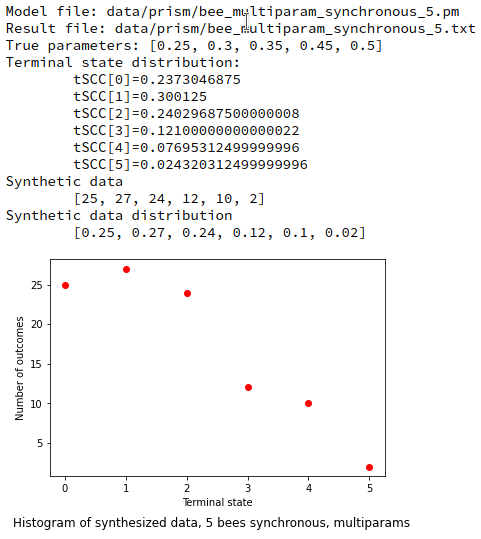
\includegraphics[width=0.5\textwidth,keepaspectratio]{figures/data_synthesis.png}
  \caption{Example of data synthesis for 5 bees model.}
\end{figure}

\subsection{Evaluation measures}
In order to evaluate the inference result, we consider three aspects:
\begin{enumerate}
\item \textit{Accuracy:} distance from estimated parameter to true parameter
  used to synthesize sample data.
\item \textit{Precision:} width of the Highest Posterior Density corresponding
  to an estimation.
\item \textit{Cost:} how does physical computation time increases as the size of
  population increases.
\end{enumerate}

To measure \textit{accuracy}, the distance from estimated parameter to true parameter, we use \textit{Root
Mean-Squared Error}.
\begin{definition}[Root Mean-Square Error]
  Let $\theta = (\theta_1,\ldots,\theta_n)$ and $\hat{\theta} =
  (\hat{\theta_1},\ldots,\hat{\theta_n})$ be vectors of $n$ real numbers, the
  Root Mean Square Error between $p$ and $\hat{p}$ is defined as follow:
  \begin{align*}
    RMSE(\theta, \hat{\theta}) = \sqrt{\frac{\sum_{i=1}^n{(\theta_i - \hat{\theta_i})}}{n}}
  \end{align*}

In the following experiments, we use the three measures (\textit{accuracy},
\textit{precision}, and \textit{cost}) to evaluate inference results.
\end{definition}

\subsection{Inference of terminal state distribution}
\subsubsection{Experiment setup}
This experiment is conducted on multiparameters, synchronous model of 5 bees.
\begin{itemize}
\item \textbf{Model file:} \texttt{bee\_multiparams\_synchronous5.pm}
\item \textbf{PRISM result file:} \texttt{bee\_multiparams\_synchronous5.txt}
\item \textbf{True parameter:} \texttt{[0.25, 0.3, 0.35, 0.45, 0.5]}
\item \textbf{True tSCC distribution:} \texttt{[0.2373046875, 0.300125,
    0.240296875, 0.1210, 0.076953125, 0.0243203125]}
\end{itemize}
In order to compare with the work by \cite{hajnal2019data}, we also visualize
the interval calculated by the following formula:
\begin{align*}
  \theta_i \pm (z_{\alpha / 2}\sqrt{\frac{\theta_i(1-\theta_i)}{N}})
\end{align*}
where $N$ is the sample size. We setup the experiment as follow:
\begin{enumerate}
\item Generate a sample terminal state data of 10 experiments.
\item Estimate terminal states distribution using Bayesian
\item Estimate terminal states and frequentist approach using accummulated data.
\item Visualize the estimated terminal state distribution from both Bayesian and
  Frequentist approach.
\item Go back to 1.
\end{enumerate}

\subsubsection{Results}
The following results are from experiment with 5 bees model. Blue line
segments visualize result from Bayesian conjugation. Green line segments
visualizes result from Frequentist approach. The blue (green) slash in the
middle of each line segment visualize corresponding point estimation.
\begin{figure}[H]
  \centering
  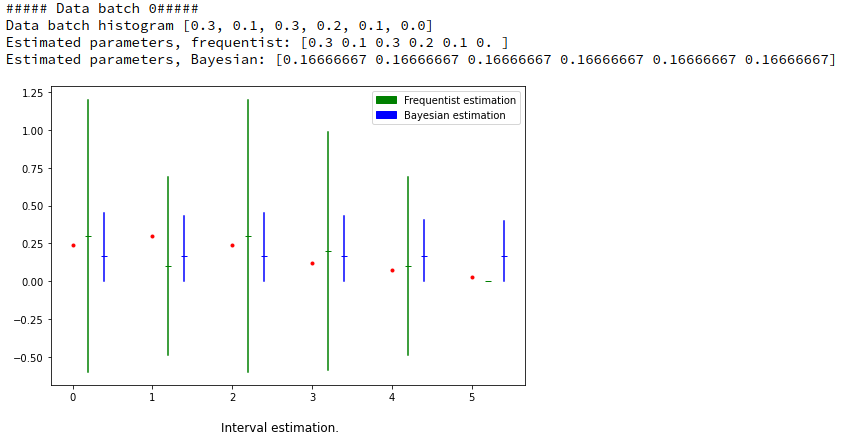
\includegraphics[width=0.8\textwidth,keepaspectratio]{figures/ex1_1.png}
  \caption{First batch of data. The Bayesian conjugation method suffers from
    initial false beliefs.}
\end{figure}

\begin{figure}[H]
  \centering
  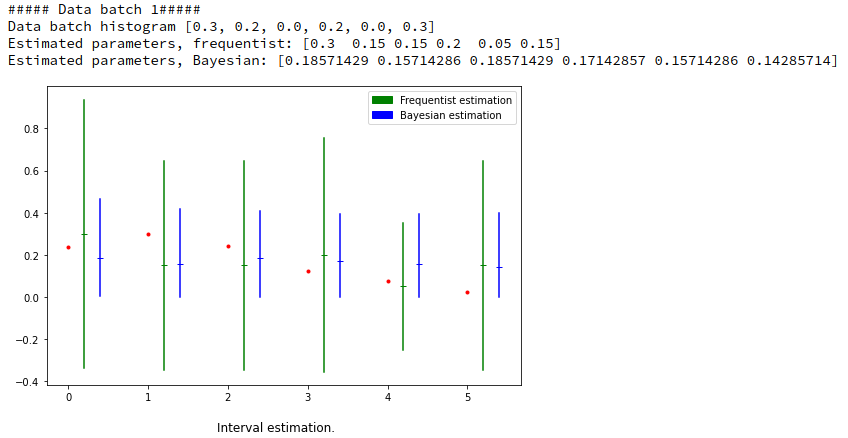
\includegraphics[width=0.8\textwidth,keepaspectratio]{figures/ex1_2.png}
  \caption{Second batch. Estimation changes significantly as we have a prior
    belief from previous batch.}
\end{figure}

\begin{figure}[H]
  \centering
  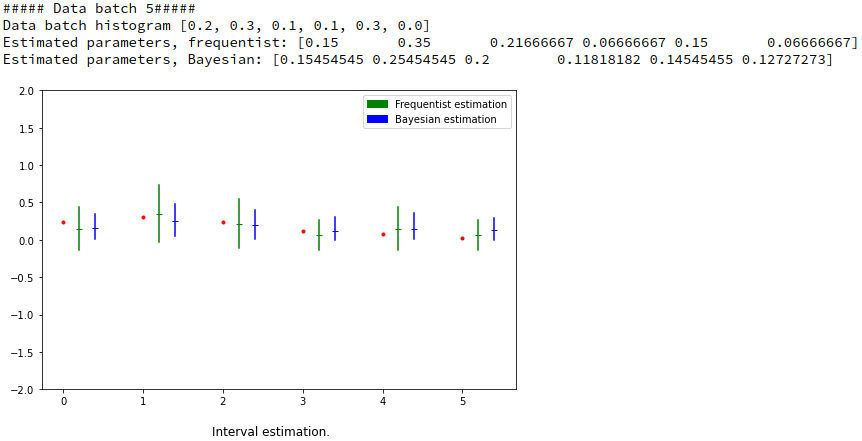
\includegraphics[width=0.8\textwidth,keepaspectratio]{figures/ex1_3.png}
  \caption{Sixth batch. Estimation improved; Bayesian Credible Sets are narrower.}
\end{figure}

\begin{figure}[H]
  \centering
  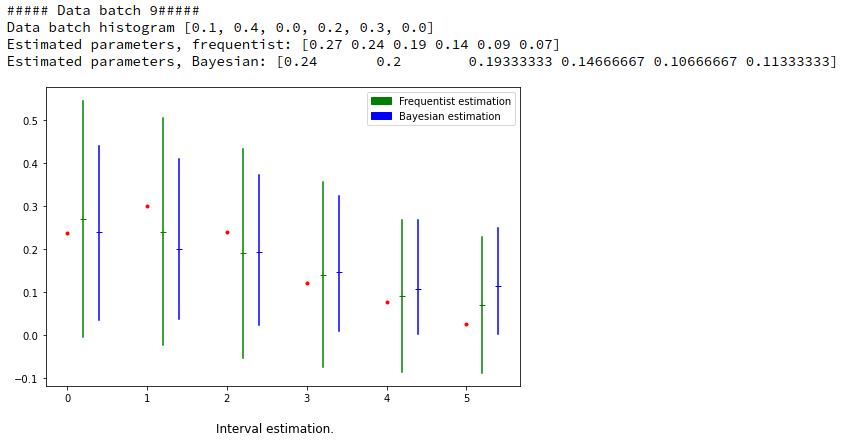
\includegraphics[width=0.8\textwidth,keepaspectratio]{figures/ex1_4.png}
  \caption{Tenth batch. At this batch, the difference between Bayesian and
    frequentist estimation is not significant, as now long-run property is satisfied.}
\end{figure}

\subsubsection{Conclusion}
With Bayesian Conjugation Multinomial-Dirichlet, we can estimate more precise
terminal state distribution than relying only on long-run property as in
frequentist approach.

\subsection{Compare DTMC sampling and rational functions}
\subsubsection{Experiment setup:}
Given different models and their corresponding (synthesized) true parameters, we
compare the accuracy and cost of estimating terminal state distribution by DTMC
sampling and rational functions evaluation.
\begin{enumerate}
\item Multiparameters, synchronous, 3 bees
  \begin{itemize}
  \item Model: \texttt{bee\_multiparams\_synchronous\_3.pm}
  \item Rational functions: \texttt{bee\_multiparams\_synchronous\_3.txt}
  \item True parameters: \texttt{[0.13816683073844171, 0.43244787684875174, 0.9883355614905787]} 
  \end{itemize}
\item Multiparameters, synchronous, 5 bees
  \begin{itemize}
  \item Model: \texttt{bee\_multiparams\_synchronous\_5.pm}
  \item Rational functions: \texttt{bee\_multiparams\_synchronous\_5.txt}
  \item True parameters: \texttt{[0.07309162012783865, 0.0732745394348604,
      0.3454227397545041, 0.5755326160799704, 0.7400394821424422]}
  \end{itemize}
\item Multiparameters, synchronous, 10 bees
  \begin{itemize}
  \item Model: \texttt{bee\_multiparams\_synchronous\_10.pm}
  \item Rational functions: \texttt{bee\_multiparams\_synchronous\_10.txt}
  \item True parameters: \texttt{[0.0010163431033164416, 0.14606188527823205,
      0.21868312430906223, 0.29198765300886687, 0.36577363178466926,
      0.48812228794389945, 0.5244272612264091, 0.7505607627245182,
      0.8753562816925659, 0.9045785878228252] }
  \end{itemize}
\item Multiparameters, synchronous, 15 bees
  \begin{itemize}
  \item Model: \texttt{bee\_multiparams\_synchronous\_15.pm}
  \item Rational functions: \texttt{bee\_multiparams\_synchronous\_15.txt}
  \item True parameters: \texttt{[0.06187489978768601, 0.08936613780246316,
      0.10191039750975828, 0.3515471096412084, 0.5311583575817167,
      0.5652253809036302, 0.6564729149073196, 0.6672538977242365,
      0.6715846867598035, 0.7099157316864673, 0.7108067756300934,
      0.7839472728483634, 0.8458734212454695, 0.853911885975256,
      0.8668668044007563]}
  \end{itemize}
\end{enumerate}
Evaluation by DTMC sampling is conducted with sample size of $2000, 4000, 8000,
10000$. We show that the distance between rational function evaluation and DTMC
sampling reduces as the sample size increases.

\subsubsection{Results}
Detailed evaluation results is logged to
\texttt{example/log/evidence/compare\_eval\_methods\_log.txt}. In this report,
first we observe the distance measured in RMSE between estimation by DTMC
sampling and rational functions evaluation.

\begin{table}[H]
  \begin{tabular}{|l|l|l|l|l|}
    \hline
    Model   & 2000 samples          & 4000 samples          & 8000 samples          & 10000 samples         \\ \hline
    3 bees  & 0.00722 & 0.00582 & 0.01149 & 0.00356 \\ \hline
    5 bees  & 0.00319 & 0.00347 & 0.00176 & 0.00269 \\ \hline
    10 bees & 0.00515 & 0.00523 & 0.00212 & 0.00213 \\ \hline
    15 bees & 0.00321 & 0.00162 & 0.00182 & 0.00181 \\ \hline
  \end{tabular}
  \caption{RMSE distance between estimation by DTMC sampling and rational functions evaluation.}
\end{table}

\begin{figure}[H]
  \centering
  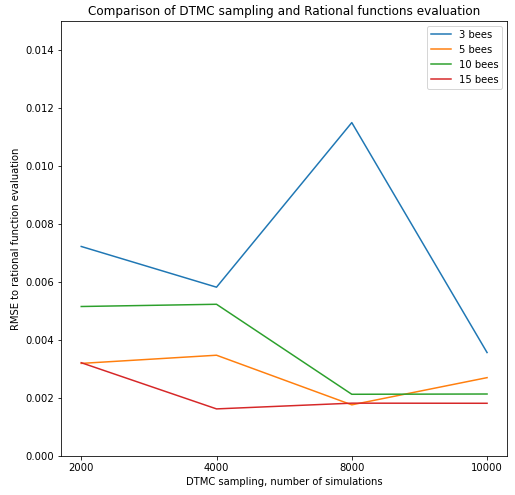
\includegraphics[width=0.5\textwidth,keepaspectratio]{figures/ex2_1.png}
  \caption{RMSE distance between estimation by DTMC sampling and rational functions evaluation.}
\end{figure}

As the results show, as we do DTMC sampling with more chain simulations, the
distance between DTMC sampling and rational functions evaluation decreases as a
result from long-run property.

\begin{table}[H]
  \begin{tabular}{|l|l|l|l|l|l|}
    \hline
    Model   & Rational function  & 2000 samples & 4000 samples  & 8000 samples  & 10000 samples  \\ \hline
    3 bees  & 0.000396   & 0.222496  & 0.318133 & 0.625835 & 0.955569 \\ \hline
    5 bees  & 0.004574   & 0.349875  & 0.427233 & 0.870164 & 0.923021 \\ \hline
    10 bees & 0.070688   & 0.990263  & 1.527305 & 2.642697 & 4.104111 \\ \hline
    15 bees & 2.935404   & 28.32838  & 47.95574 & 86.77052 & 104.0558 \\ \hline
  \end{tabular}
  \caption{Physical runtime comparison, measured in seconds}
\end{table}

The rational function evaluation time can be reduced by factorizing rational
functions to their simpler form with the help of \cite{meurer2017sympy}. \\
\begin{table}[H]
  \begin{tabular}{|l|l|l|l|l|l|}
    \hline
    Model   & Non-factorized  & Factorized  \\ \hline
    3 bees  & 0.000396   & 0.000368 \\ \hline
    5 bees  & 0.004574   & 0.000744 \\ \hline
    10 bees & 0.070688   & 0.036026 \\ \hline
    15 bees & 2.935404   & 1.215543 \\ \hline
  \end{tabular}
  \caption{Physical runtime comparison of evaluation non-factorized and
    factorized rational functions, measured in seconds}
\end{table}

The time needed to process rational functions with factorization
increases exponentially to the footprint of rational functions. 
\begin{table}[H]
  \begin{tabular}{|l|l|l|l|l|l|}
    \hline
    Model   & Non-factorized rational functions & Factorized rational functions \\ \hline
    3 bees  & 0.002133   & 0.040748 \\ \hline
    5 bees  & 0.024780   & 0.167829 \\ \hline
    10 bees & 0.326980   & 20.498155 \\ \hline
    15 bees & 8.906071   & 10649.155044 \\ \hline
  \end{tabular}
  \caption{Physical runtime comparison of parsing rational functions, with and
    without factorization, measured in seconds}
\end{table}
It must be noticed that the cost of factorization, while very high, is paid only
once at the model processing, an later the reduction in rational functions
evaluation is significant, as the number of rational functions evaluation is
linear to the Metropolis-Hastings chain length.

\subsubsection{Conclusion}
DTMC sampling can be used as an alternative method for terminal state
distribution evaluation. It is due to the long-run property that as we do more
chain simulations, the estimated terminal state distribution becomes closer to
the distribution evaluated from rational functions. DTMC sampling has a
significant advantage that it does not need a symbolic model checker to deliver
rational functions; it also eliminates the overhead that is induced by reading
and parsing large rational functions.


\subsection{Inference of model parameters}
\subsubsection{Experiment setup}
We shows examples of parameter inference for different bees model in both DTMC
sampling and rational functions evaluation methods. Other setups:
\begin{itemize}
\item Prior distribution: $Uniform(0, 1)$
\item Metropolis-Hastings chain length: $500$
\item Number of simulations in DTMC sampling mode: $1000$.
\end{itemize}

\subsubsection{Results}
Results compiled from log file \texttt{examples/logs/evidences/run_normal_log.txt}.\\
Results with 3 bees model, multiparameters, synchronous.
Results with 5 bees model, multiparameters, synchronous.
Results with 10 bees model, multiparameters, synchronous.
Results with 15 bees model, multiparameters, synchronous.
For large population models which due to the technical issues PRISM cannot
deliver rational functions, we can only use DTMC sampling to estimate terminal
state. However, as it has been shown on the comparison betwwen rational function
evaluation and DTMC sampling, cost for a DTMC simulation also increases as the
number of states in the DTMC increases.\\

\subsubsection{Conclusion}
The experiment shows the results on parameter inferecence for agnostic models of
3, 5, 10, and 15 bees.


\subsection{Selection of Metropolis-Hastings chain length}
\subsubsection{Experiment setup}
Chain length in Metropolis-Hastings algorithm is the number of accepted point
that is added to the sample set, which is returned by the algorithm. In this
experiment we evaluate the impact of different Metropolis-Hastings chain length
to parameter estimation.\\
We use 10 bees, multiparameterrs, synchronous model. Using the same true
parameter and synthetic data, we do the parameter inference in different
Metropolis-Hastings trace length, and observe the changes in parameter
estimation.
\begin{itemize}
\item Model: 10 beesm, 
\end{itemize}
\subsubsection{Result}
Results compiled from log file \texttt{examples/logs/evidences/compare_mcmc_chainlen_log.txt}.\\
Precision of inference results with different Metropolis-Hastings chain length in
the set $(1000, 2000, 3000, 4000, 5000)$ is visualized in the following figure. 
\begin{figure}[H]
  \centering
  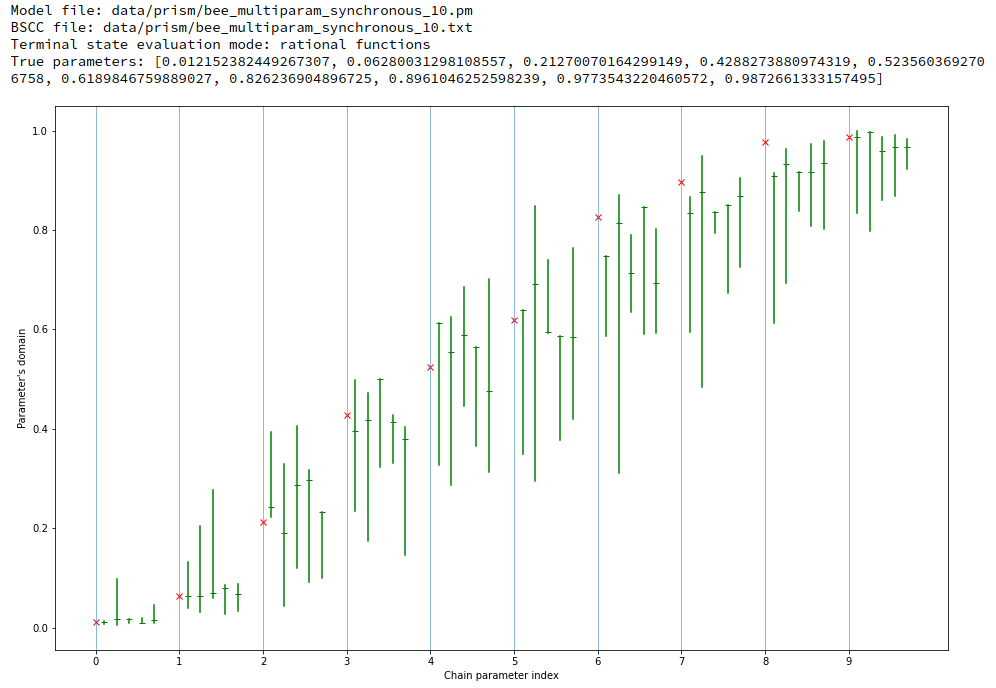
\includegraphics[width=\textwidth,keepaspectratio]{figures/compare_mcmc_chainlength.png}
  \caption{HPD of inference result. Green lines from left to right visualize the
  HPD of inference with Metropolis-Hastings chain length $1000, 2000, 3000,
  4000, 5000$. The red cross visualizes true parameter.}
\end{figure}
Accuracy and runtime:
\begin{table}[H]
  \begin{tabular}{|l|l|l|}
    \hline
    MH Chainlength & RMSE                 & Run time (s) \\ \hline
    1000           & 0.050052749138867626 & 63.83112     \\ \hline
    2000           & 0.03084112520832641  & 125.08478    \\ \hline
    3000           & 0.0601108203086657   & 183.794119   \\ \hline
    4000           & 0.04131949555520387  & 246.105021   \\ \hline
    5000           & 0.051880135378818214 & 306.694507   \\ \hline
  \end{tabular}
  \caption{Accuracy (measured by RMSE) and run time (in seconds), inference of
    10 bees, multiparameters, synchronous model with different
    Metropolis-Hastings chain length.}
\end{table}

\subsubsection{Conclusion}
From the results of experiment, we cannot conclude that increasing
Metropolis-Hastings chain length also increases parameter estimation accuracy.
It is because that there are too many outliers in the results. However, as it
can be seen from the visualization, increase the Metropolis-Hastings
chainlength, in general, can improve the precision of the inference.

\subsection{Selection of prior distribution}
\subsubsection{Experiment setup}
Results compiled from log file \texttt{examples/logs/evidences/compare_prior_log.txt}.\\
This experiment is to show the impact of prior distribution selection on a given
bees model. In this particular setup, we compare $Uniform(0,1)$ and
$Beta(\alpha, \beta)$. Other settings: 
\begin{itemize}
\item Metropolis-Hastings chain length: $500$
\item Terminal state distribution evaluation: rational functions evaluation.
\end{itemize}

\subsubsection{Result}


\subsubsection{Conclusion}
As the results show, the selection of prior distribution has a strong impact on 
For example, in the case of linear model, certain assumption can be made on
model parameters so that we can limit the parameter space. 

\subsection{Impact of data quality}
\subsubsection{Experiment setup}
An advantage of using synthetic data over real data obtained from biological
experiment is that:
\begin{itemize}
\item We know the true parameters.
\item We have control over data quality.
\end{itemize}
Biological experiment, in this project is the experiment with bees, is not able
to be conducted massively, for example $1000$ experiments, due to the time and
effort cost. To few experiments to guarantee the long-run property leads to
incorrect parameter inference. In this experiment, we evaluate the impact of
low quality data (too few experiment data) to parameter inference. 
Experiment is conducted as follow
\begin{itemize}
\item 
\end{itemize}
\subsubsection{Result}

Results compiled from log file \texttt{examples/logs/evidences/compare_data_quality_log.txt}.\\
\subsubsection{Conclusion}

\subsection{Linear model}
\subsubsection{Experiment setup}
Linear models use the same model sematics to multiparameters model. The
difference is that it assume that parameters are linearly related.
\begin{enumerate}
\item Multiparameters, synchronous, 5 bees
  \begin{itemize}
  \item Model: \texttt{bee\_multiparams\_synchronous\_5.pm}
  \item Rational functions: \texttt{bee\_multiparams\_synchronous\_5.txt}
  \item True parameters: \texttt{[0.1, 0.2]}
  \item Synthetic data ($10000$ trials): \texttt{[3253, 2421, 1763, 1257, 870, 436]}
  \end{itemize}
\item Multiparameters, synchronous, 10 bees
  \begin{itemize}
  \item Model: \texttt{bee\_multiparams\_synchronous\_10.pm}
  \item Rational functions: \texttt{bee\_multiparams\_synchronous\_10.txt}
  \item True parameters: \texttt{[0.01, 0.02]}
  \item Synthetic data ($10000$ trials): \texttt{[8161, 1523, 267, 46, 3, 0, 0, 0, 0, 0, 0]}
  \end{itemize}
\end{enumerate}

As linear constraint in linear model imposes that $r_i = a\times i + b$, in
which $a$ and $b$ are model parameters. This results in two important observations on
prior distribution:
\begin{enumerate}
\item Values range in $[0,1]$
\item Strongly skewed to small values of $a$ and $b$ in range $[0,1]$, otherwise it results in
  $r_i>1$, which is invalid.
\end{enumerate}
Using these observations as our prior beliefs, we select the distribution
$Beta(\alpha=1,\beta=10)$ as prior distribution.
\begin{figure}[H]
  \centering
  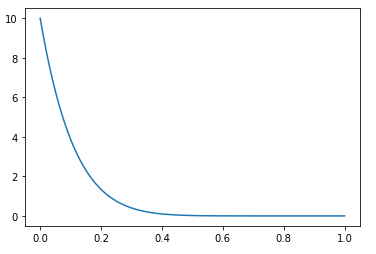
\includegraphics[width=0.5\textwidth,keepaspectratio]{figures/beta_1_10.png}
  \caption{$Beta(\alpha=1,\beta=10)$ prior distribution. The distribution is
    skewed to lower values of rang $[0,1]$.}
\end{figure}

\subsubsection{Results}
The following results are from experiment with 5 bees  and 10 bees models. The
green bars visualize HPD of estimations, with a dash in betwwen to visualize the
point estimation.
\begin{figure}[H]
  \centering
  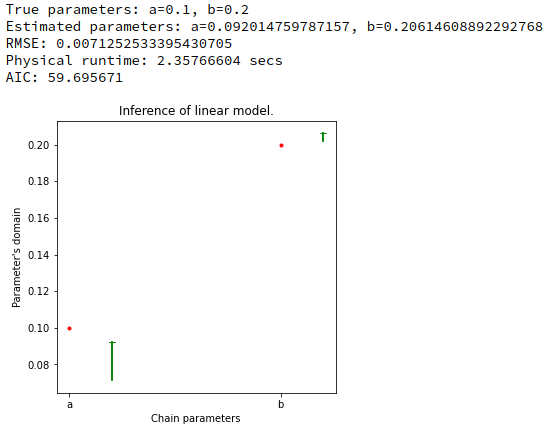
\includegraphics[width=0.7\textwidth,keepaspectratio]{figures/linear_1.png}
  \caption{Inference of Linear 5 bees model.}
\end{figure}
Result with 10 bees model.
\begin{figure}[H]
  \centering
  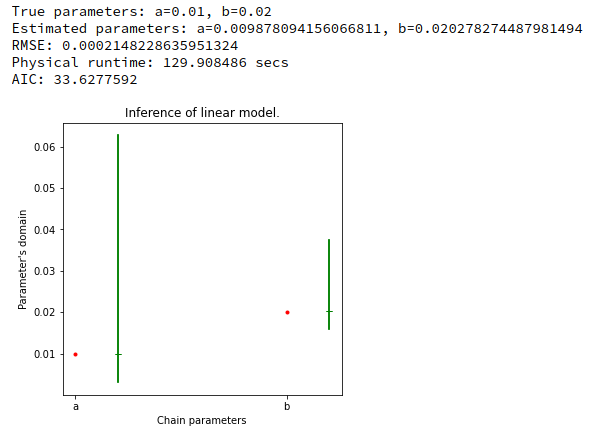
\includegraphics[width=0.7\textwidth,keepaspectratio]{figures/linear_2.png}
  \caption{Inference of Linear 10 bees model.}
\end{figure}

\subsubsection{Conclusion}
Linear model helps to reduce the number of model parameters by enforcing a
linear constraint, thus all multiparameters model reduced into 2 parameters.
With the proper selection of prior distribution to avoid too many invalid
parameter evaluation, parameters of linear models can be estimated with high
likelihood and relatively cheap physical runtime cost.

%%%%%%%%%%%%%%%%%%%%%%%%%%%%%%%%%%%%%%%%%%%%%%%%%%%%%%%%%%%%%%%%%%%%%%%%%%%%%%%%%%%%%%%%%%
\section{Implementation}
\subsection{Class design}
\begin{figure}[H]
  \centering
  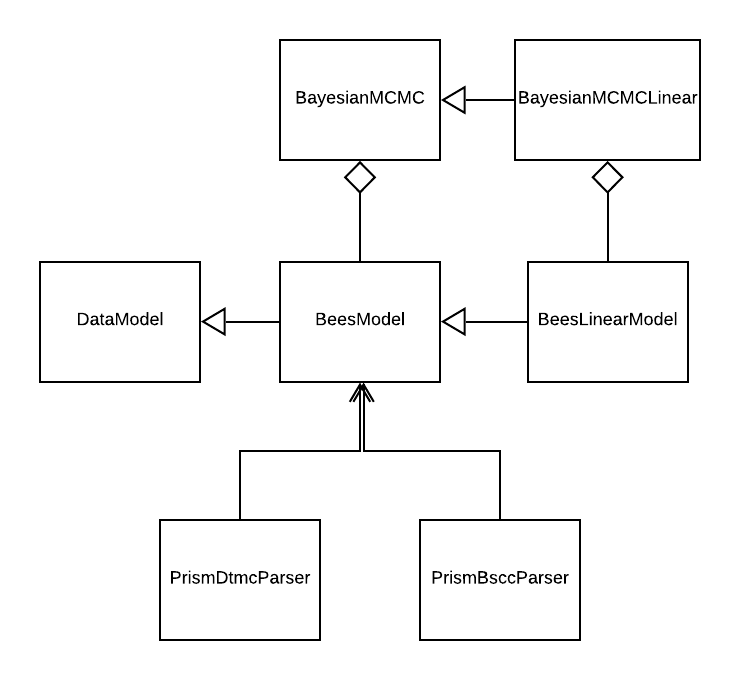
\includegraphics[width=0.6\textwidth,keepaspectratio]{figures/class_diagram.png}
  \caption{Class diagram of the project}
\end{figure}
Class explanation:
\begin{enumerate}
\item \texttt{PrismModelParser} and \texttt{PrismBsccParser} parses PRISM model
  file and symbolic model checking results. In details, the two classes do the
  following tasks:
  \begin{itemize}
  \item Read PRISM model and result files.
  \item Extract and preprocess expressions from model and result.
  \item Factorize expressions if needed
  \item Parse expressions in model and result file. store in Python bytecode.
  \item Create \texttt{DataModel} object to store these parsed expressions.
  \end{itemize}
\item \texttt{DataModel}, \texttt{BeesModel}, and \texttt{BeesLinearModel} store
  information about the population model.
\item \texttt{BayesianMcmc} and \texttt{BayesianMcmcLinear} implements
  Metropolis-Hastings algorithm.
\end{enumerate}

\subsection{Test environment}
The Bayesian inference methods are implemented in Python 3 and tested in the
followin system configuration:
\begin{itemize}
\item Intel Core i5-8265U @ 1.60GHz
\item 16GB RAM
\item OpenSUSE Tumbleweed 20200427
\item Anaconda 3 2019.10 for linux x86\_64
\end{itemize}

\subsection{Directory structure}
\begin{itemize}
\item \texttt{data} folder contains PRISM models and model checking results.
\item \texttt{docs} folder contains final report
\item \texttt{scripts} folder contains python implementation.
\item \texttt{examples} folder contains experiment schemes.
  \begin{itemize}
  \item \texttt{examples/evidence} contains log of the examples that are used as
    data for this report.
  \end{itemize}
\end{itemize}


%%%%%%%%%%%%%%%%%%%%%%%%%%%%%%%%%%%%%%%%%%%%%%%%%%%%%%%%%%%%%%%%%%%%%%%%%%%%%%%%%%%%%%%%%% 
\section{Conclusion}
The goal of this project is to experiment Bayesian approach on parameter
inference of Markov population models. The results shows that Bayesian inference
is efficient to deliver an estimation of model parameters. Given that in the
biological system that is modelled, each parameters represent a real-world
biological property, such as the probability of a bee sting, given a certain
amount of pheromone, the parameter estimation presented in this project helps
biologists to better understand the biological mechanism.\\

The implementation in this project is capable of estimating parameters in both
cases, when rational functions are available and is not available. This is an
advantage in case that model checker cannot deliver rational functions due to
technical issues. Also, with the parallelization of DTMC sampling, the
implementation proves that it has significant scalability for models of large
populations. The implementation also works with linear models and 2 parameters
model, with significant reduction of physical runtime.\\

While the implementation in this project only gives point estimations and their
corresponding credible set, the parameter synthesis method presented in
\cite{hajnal2019data} gives a detailed analysis of accepted regions and rejected
regions on parameter space and does not need to manually select a proper prior
distribution. We suggest that the implementation in this project should be
intergrated to the tool DiPS in \cite{hajnal2019data} as an extension, so user
can use it as an option. By doing so, we can exploit the advantages of both
methods depend on particular situations.\\
There are still problems, which are not completely solved in the scope of this
project:
\begin{enumerate}
\item \textit{Number or parameters}: Accuracy and precision of an estimation
  decreases, while the computational cost increases, as the number of model
  parameter increases.
\item \textit{Selection of prior:} a false selection of prior distribution and
  its parameters could propagate false beliefs over the whole inference. So far
  we have been using Uniform distribution by default to prevent 
  This project has not coped with the problem of hyperparameters
  estimation.
\item Using \textit{STORM} \cite{dehnert2017storm} as a more effective model
  checker in stead of PRISM. STORM is capable of handling rational functions
  with larger footprint and factorizing these functions. However due to
  technical problems and time constraint, \textit{STORM} is not used in this
  project.
\item There is still a problem of number overflow that appears randomly in case
  of evaluation of parametric DTMC in large model (for example, 20 bees
  multiparameters, synchronous). However, the root cause of this issue is
  unknown and thus it is not solved.
\end{enumerate}

%%%%%%%%%%%%%%%%%%%%%%%%%%%%%%%%%%%%%%%%%%%%%%%%%%%%%%%%%%%%%%%%%%%%%%%%%%%%%%%%%%%%%%%%%% 
\newpage
\printbibliography

\end{document}


